% Template for Cogsci submission with R Markdown

% Stuff changed from original Markdown PLOS Template
\documentclass[10pt, letterpaper]{article}

\usepackage{cogsci}
\usepackage{pslatex}
\usepackage{float}
\usepackage{caption}

% amsmath package, useful for mathematical formulas
\usepackage{amsmath}

% amssymb package, useful for mathematical symbols
\usepackage{amssymb}

% hyperref package, useful for hyperlinks
\usepackage{hyperref}

% graphicx package, useful for including eps and pdf graphics
% include graphics with the command \includegraphics
\usepackage{graphicx}

% Sweave(-like)
\usepackage{fancyvrb}
\DefineVerbatimEnvironment{Sinput}{Verbatim}{fontshape=sl}
\DefineVerbatimEnvironment{Soutput}{Verbatim}{}
\DefineVerbatimEnvironment{Scode}{Verbatim}{fontshape=sl}
\newenvironment{Schunk}{}{}
\DefineVerbatimEnvironment{Code}{Verbatim}{}
\DefineVerbatimEnvironment{CodeInput}{Verbatim}{fontshape=sl}
\DefineVerbatimEnvironment{CodeOutput}{Verbatim}{}
\newenvironment{CodeChunk}{}{}

% cite package, to clean up citations in the main text. Do not remove.
\usepackage{apacite}

% KM added 1/4/18 to allow control of blind submission
\cogscifinalcopy

\usepackage{color}

% Use doublespacing - comment out for single spacing
%\usepackage{setspace}
%\doublespacing


% % Text layout
% \topmargin 0.0cm
% \oddsidemargin 0.5cm
% \evensidemargin 0.5cm
% \textwidth 16cm
% \textheight 21cm

\title{No evidence for familiarity preferences after partial exposure to
visual concepts in preschoolers and infants}


\author{Gal Raz$^1$ (galraz@mit.edu), \bf{Anjie Cao$^2$  (anjiecao@stanford.edu)},\\ \bf{Minh Khong Bui$^3$  (mbui100@csu.fullerton.edu)}, \\ \bf{Michael C. Frank$^2$ (mcfrank@stanford.edu)},
 and \bf{Rebecca Saxe$^1$ (saxe@mit.edu)} \\
$^1$Department of Brain and Cognitive Sciences, MIT, $^2$Department of Psychology, Stanford University, \\ $^3$Department of Communicative Sciences and Disorders, California State University \\ }

\newlength{\cslhangindent}
\setlength{\cslhangindent}{1.5em}
\newenvironment{CSLReferences}%
  {}%
  {\par}

\begin{document}

\maketitle

\begin{abstract}
From birth, humans constantly make decisions about what to look at and
for how long. A classic framework of information-seeking in development
proposes encoding as a key driver of looking behavior - in early stages
of encoding, infants and young children will prefer to engage with
familiar stimuli in order to complete their representation, while at
later stages of encoding they will preferentially attend to novel
stimuli. While this framework is often invoked in the interpretation of
looking times studies, it is rarely explicitly validated empirically.
Here, we test these predictions using new paradigms which manipulate
exposure durations to different stimuli within-subjects. While we find
robust evidence for habituation and novelty preferences across
development, limiting exposure to visual concepts did not result in
familiarity preferences in any age group. Our findings suggest that
limited exposure does not generically lead to familiarity preferences in
sequential paradigms, and that interpretations of observed familiarity
preferences should be made with care. We argue for the development of
formal, predictive frameworks which link the learning problem faced by
participants to their attentional preferences.

\textbf{Keywords:}
psychology; development; learning
\end{abstract}

\hypertarget{introduction}{%
\section{Introduction}\label{introduction}}

Throughout development, humans are inundated with visual information.
Infants and young children constantly decide how much time to spend
looking at what is in front of them and when to move on to something
else (Dweck, 2017; Haith, 1980; Raz \& Saxe, 2020). Developmental
psychologists have long relied on infants' ability to decide what to
look at and for how long, to make inferences about infants' mental
representations (Aslin, 2007; Baillargeon, Spelke, \& Wasserman, 1985;
Fantz, 1963). In a typical study measuring looking time, infants are
presented with the same stimulus repeatedly until their looking time
decreases (i.e.~habituation). Then, they are presented with a new
stimulus, and the change in their looking time is used as evidence for
cognitive capacities. Despite extensive use of looking time as a
measure, the rules underlying infants' decision to keep looking or look
away are not well understood. In this paper, we conduct a direct
empirical test of the relationships between prior exposure and looking
preferences.

One dominant framework for infant looking is that the dynamics of
looking time are governed by the dynamics of learning (Hunter \& Ames,
1988). This framework has been used to derive qualitative predictions
about looking time as a function of prior exposure and stimulus
complexity. If infants have sufficient prior exposure to complete
encoding of one stimulus, they should look longer at a novel stimulus
that offers new opportunities to learn, showing a novelty preference. In
contrast, when infants have only limited prior exposure or have
partially encoded one stimulus, they might look at that same stimulus
for longer to learn more about it, showing a familiarity preference.

However, empirical studies that systematically quantify familiarity
preferences for visual stimuli tend to be older, have smaller sample
sizes, and limited or no data available, making them unsuitable for
evaluating the robustness of the phenomenon (e.g.: Hunter, Ames, \&
Koopman, 1983; Rose, Gottfried, Melloy-Carminar, \& Bridger, 1982).
Furthermore, this theoretical framework does not include formal criteria
to judge the completeness of encoding, limiting the precision of
predictions for new experiments. The dynamics in this framework are
instead often invoked retroactively, to explain unexpected findings. For
example, Johnson et al. (2009) studied rule learning in 8- and 11-month
old infants, finding a novelty preference in 8-month olds in one
condition and a familiarity preference in 11-month olds in three others
(as well as four conditions with no significant differences). They
interpreted these differences post hoc as indicating some combination of
greater complexity for certain rules over others and faster encoding by
older children.

To move from post hoc interpretations towards predictive frameworks of
looking time experiments, computational models are beginning to play a
role. Across the cognitive sciences, computational models facilitate
theory-building and provoke more precise formulations of cognitive
phenomena (Guest \& Martin, 2021; Smaldino, 2020). For infant looking,
formal models of learning have successfully predicted infants'
habituation and subsequent preferences for novel stimuli. However, in
contrast to Hunter \& Ames (1988)'s framework, these formal models
generally do not predict that infants will show a familiarity preference
when given limited learning experience (Sirois \& Mareschal, 2002). In a
recent example of such a model, Cao, Raz, Saxe, \& Frank (2022) proposed
that habituation and novelty preference could be explained by a rational
learner that takes noisy perceptual samples to maximize information gain
(RANCH: Cao et al., 2022). This model accurately predicted adult looking
time patterns in a self-paced habituation paradigm, reproducing both
habituation and novelty preferences. However, RANCH did not predict
familiarity preferences at any stage of encoding, because its learning
policy to maximize information gain would always prioritize learning
about a novel stimulus over a repeated familiar stimulus, just to
varying degrees.

By contrast, other models do seem to contain either indirect or direct
predictions of familiarity preference. Kidd, Piantadosi, \& Aslin (2012)
proposed the ``Goldilocks effect'' -- infants' tendency to focus on
things that are neither too simple nor too complex - as a formal account
of infant looking. In this work, an ideal learner model tracked the
relative probability of objects appearing in specific locations in a
continuous stream of events, and infants' probability of looking away
from each successive object had a U-shaped link to the models'
surprisal. It has been suggested that infants' tendency to stay most
engaged with moderately predictable events may be a reflection of
familiarity preferences at early stages of encoding. A more recent
formal model used rational information gathering agents to explain
infant looking behaviors, and directly predicted familiarity preferences
(Karni, Mattar, Emberson, \& Daw, 2022). This model is similar to RANCH
in that its learning policy considers information gain, but it also
considers another source of value (i.e.~information ``need'': how
frequently the information about each stimulus will be used). A
trade-off between information gain and information need generates
non-monotonic changes in looking time, which predict both familiarity
preferences and novelty preferences. To evaluate and compare the
predictions of these different model types, it is necessary to have
quantitative estimates of habituation, novelty preferences, and
familiarity preferences in infants. Under what circumstances do infants
look longer at a stimulus, following limited exposure and thus
potentially partial encoding?

In this paper, we aim to offer a stronger empirical foundation for
understanding how the duration of exposure influences looking duration.
We conducted experiments with preschoolers and infants to test the
conditions under which a familiarity preference could be elicited. For
preschoolers, we adapted a self-paced looking time paradigm that was
previously used to capture habituation and novelty preference in adults
(Cao et al., 2022). For infants, we developed a new within-participants
measurement paradigm. This set of experiments allows us to directly
investigate whether a familiarity preference arises when learners have
limited experience with stimuli. To preview, while preschoolers and
infants show both habituation and novelty preferences in our paradigm,
we found no evidence for a familiarity preference in either preschoolers
or infants.

\hypertarget{experiment-1}{%
\section{Experiment 1}\label{experiment-1}}

Hunter \& Ames (1988) posit that younger participants are more likely to
exhibit familiarity preferences after the same amount of exposure to a
stimulus due to their reduced encoding speed. There is some empirical
evidence suggesting that younger infants show familiarity preferences in
tasks in which older infants show novelty preferences (Cyr \& Shi, 2013;
Thiessen \& Saffran, 2003). This age-related change in preference may
explain the lack of familiarity preference observed in adults (Cao et
al., 2022; Gustafsson, Francoeur, Blanchette, \& Sirois, 2021). It is
possible that adults can process so fast that even brief exposure is
sufficient for completing stimulus encoding. We therefore tested young
children on an experimental paradigm that has captured habituation and
novelty preference in adults (Fig. 1: left panel, Cao et al., 2022).

\hypertarget{methods}{%
\subsection{Methods}\label{methods}}

\hypertarget{participants}{%
\subsection{Participants}\label{participants}}

66 children completed a task modified from the adult self-paced looking
time studies reported in Cao et al. (2022). Following our
pre-registration
(\href{https://aspredicted.org/blind.php?x=5WQ_YQH}{link}), 2 children
were excluded from the analysis because their performance in the
attention-check task failed to meet the inclusion criteria (answering 4
out of the 8 attention check questions correctly). We also excluded
trials with looking time that were three absolute deviations away from
the median in the log-transformed space across participants (Total trial
\emph{N} = 3564; Excluded trial \emph{N} = 83, 2.33\% of the total
trials). The final datasets includes 64 children in total (3yr: N = 18;
4yr: N = 26; 5yr: N = 20). All participants were recruited in a
university-affiliated research preschool.

\begin{CodeChunk}
\begin{figure*}[h]

{\centering 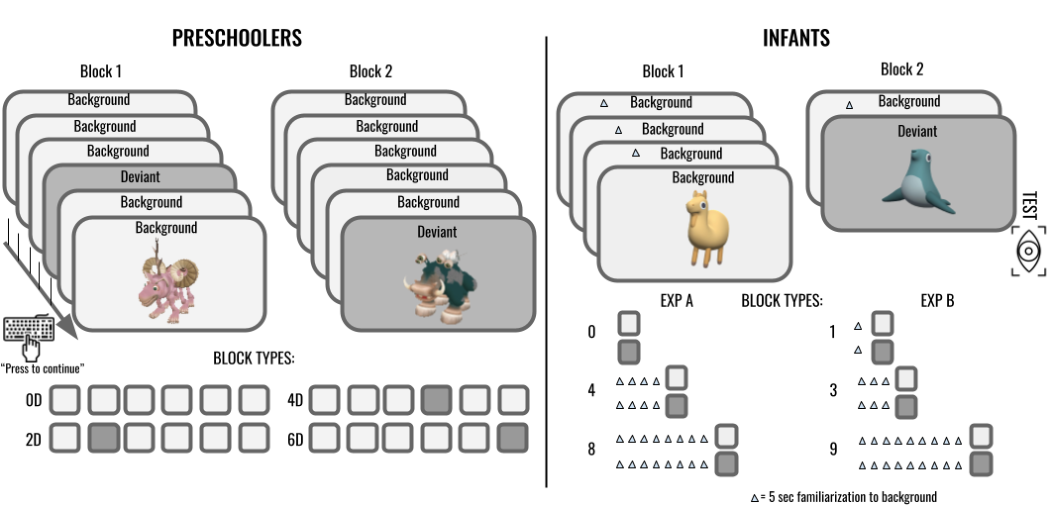
\includegraphics{figs/experimental_design-1} 

}

\caption[Experimental design of preschooler and infant experiments]{Experimental design of preschooler and infant experiments. There were four main differences: 1) Preschoolers responded with button presses, infants through lookaways, 2) preschoolers saw background trials after deviants, whereas deviants always appeared at the end in the infant experiments, 3) in preschoolers all trials were self-paced, whereas in infants only the last trial was self-paced and 4) preschooler and infant paradigms used different sets of animate stimuli.}\label{fig:experimental_design}
\end{figure*}
\end{CodeChunk}

\hypertarget{stimuli}{%
\subsection{Stimuli}\label{stimuli}}

We used a subset of stimuli used in a prior adult self-paced looking
time study, a set of animated creatures from the computer game Spore
(developed by Maxis in 2008).

\hypertarget{procedures}{%
\subsection{Procedures}\label{procedures}}

Children were tested individually in a test room by an experimenter. The
experimenter invited the child to ``meet some monster friends'\,' and
then familiarized the child with the laptop computer used to present the
experiment. Before the test, each child went through a practice phase
where they practiced pressing the space bar to move on to the next
trial. The child was instructed that they can press the key and move on
to meet more monster friends whenever they want.

On each trial, the child would see an animated creature appear on the
screen. The child could move on to the next trial by pressing the space
bar. Each block consisted of six trials. Usually, the same creature was
shown repeatedly (the background stimulus), but each block could contain
either zero or one deviant trial. Deviant trials were trials that
present a different creature from the background stimulus. Deviant
trials appeared on the second, the fourth, or the sixth trial of the
block. Each child saw eight blocks in total.

At the offset of each block, we presented a memory task to ensure
children were appropriately attending to the task, asking them which of
two creatures they had seen before.

\hypertarget{results}{%
\subsection{Results}\label{results}}

Data and analysis are available
\href{https://tinyurl.com/PokebabyCogSci2023}{here}. Children included
in the final dataset showed a high level of accuracy (\emph{M} = 0.97;
\emph{SD} = 0.08) in responding to the memory task question. This
suggests that the children were engaged in the experiment. We
anticipated that the preschooler children would show patterns of
habituation and dishabituation similar to adults. We also expected to
see developmental changes in the shape of habituation trajectories. Our
pre-registered mixed-effect model included a three-way interaction term
between age (in months; scaled and centered), trial number, and trial
type (background or deviant) to predict log-transformed looking time.
The interaction between the trial number and trial type was significant,
suggesting the paradigm has captured habituation and novelty preference
in preschoolers (\(\beta\) = 0.14, \emph{SE} = 0.02, \emph{t} = 6.22,
\emph{p} \textless{} 0.01). However, we did not find any significant
interaction with age, nor was the main effect significant (all \emph{p}
\textgreater{} 0.1).

We also tested for familiarity preferences by comparing the looking time
at the second background trial and the second deviant trial. Under the
(Hunter \& Ames, 1988) framework, the second trial in each block may be
most likely to yield a familiarity preference, since participants have
had the least amount of exposure to the background stimulus in a block.
If there was a familiarity preference, participants should look longer
at a background trial than a deviant trial. However, we did not find
evidence supporting this prediction. We ran a mixed effect model
predicting looking time at the second trial with trial type as the
predictor. There was a significant trial type effect in the opposite
direction, suggesting participants looked longer at the deviant trial
than the background trial even with as little as one trial of
familiarization time (\(\beta\) = 0.41, \emph{SE} = 0.03, \emph{t} =
12.24, \emph{p} \textless{} 0.01).

\begin{CodeChunk}
\begin{figure}[t!]

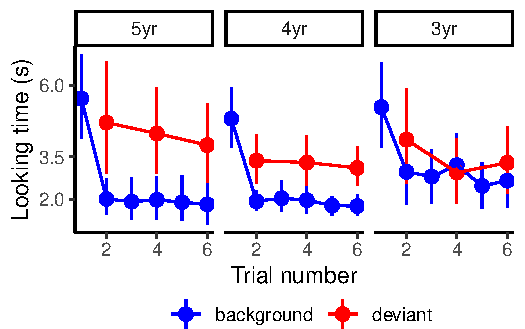
\includegraphics{figs/unnamed-chunk-13-1} \hfill{}

\caption[Looking times of preschoolers faceted by age showing habituation and dishabituation, but not familiarity preferences]{Looking times of preschoolers faceted by age showing habituation and dishabituation, but not familiarity preferences. Y-axis is log-transformed to reflect transformation of looking times in mixed effects models.}\label{fig:unnamed-chunk-13}
\end{figure}
\end{CodeChunk}

In summary, this experiment captured habituation and novelty preferences
in preschoolers, replicating the patterns seen in a previous adult
sample (Cao et al., 2022). In contrast, we did not find any evidence of
familiarity preferences. It is possible that processing in preschoolers
is already too fast for us to induce partial encoding in this paradigm.
If so, we would need to test a younger population. However, given that
the performance of 3-year-olds in this paradigm was noisier than their
older peers (Fig. 2), the current paradigm would likely not be suitable
for testing even younger children. In Experiment 2, we developed a new
experimental paradigm to measure the relationship between exposure
duration and looking preferences in preverbal infants.

\hypertarget{experiment-2}{%
\section{Experiment 2}\label{experiment-2}}

In the infant paradigm, infants are familiarized to six unique stimuli
for different exposure durations within a single session in a blocked
design (Fig. 1, right panel). This is in contrast to the standard infant
familiarization/habituation paradigm in which infants are familiarized
to only one stimulus throughout an experiment, so the effects of
exposure duration must be estimated between groups of infants. By
presenting individual infants with multiple blocks and varying exposure
times, we directly measure the effect of prior exposure on looking
times, within participants.

To get a dense sample of possible exposure durations, we pre-registered
and ran two experiments, sequentially, with two sets of exposure
durations. The first experiment showed infants blocks containg 0, 4 or 8
exposure events (Exp A; pre-registered
\href{https://osf.io/gux4f/?view_only=b4d6d0118dfa41a79fb431d389f4fecc}{here}).
The second experiment showed infants blocks containing 1, 3 or 9
exposure events (Exp B; pre-registered
\href{https://osf.io/w6pgu/?view_only=39ee108159884761a0c5bc68d11918df}{here}).

\hypertarget{methods-1}{%
\subsection{Methods}\label{methods-1}}

\hypertarget{participants-1}{%
\subsection{Participants}\label{participants-1}}

We tested a combined sample of 66 7-10 month old infants, with 31 in Exp
A and 35 in Exp B (\(M_{age}\) = 9.5 months, 31 female). 5 participants
were excluded completely due to fussiness. An additional 78 individual
test events (out of 366, 21.7\% of trials) did not make it into the
final analysis because 1) infants fussed out of the experiment at an
earlier stage of the experiment, 2) infants looked at the stimuli for
less than a total 2 seconds, 3) there were momentary external
distractions in the home of the infant or 4) the gaze classifier (see
\textbf{Looking time coding}) had an average classification confidence
of less than 50\%. Data collection was performed synchronously on Zoom,
and infants were recruited from Lookit (Scott \& Schulz, 2017) and
Facebook.

\hypertarget{stimuli-1}{%
\subsection{Stimuli}\label{stimuli-1}}

Infants saw a different stimulus set from the preschoolers. In two
initial studies, not included here, we showed infants the Spore stimulus
set used in preschoolers, in a slightly different experimental paradigm,
and failed to elicit replicable habituation, novelty or familiarity
preferences. In the current studies, we presented infants with a series
of animated animals, created using ``Quirky Animals'' assets from Unity
(Fig. 1, \href{https://tinyurl.com/469xxrn7}{link}). The animals were
walking, crawling or swimming, depending on the species.

\hypertarget{procedure}{%
\subsection{Procedure}\label{procedure}}

This experiment followed a block structure, where each block was divided
into two sections: 1) a familiarization period and 2) a test event. Each
block was preceded by our lab-standard attention getter, a salient
rotating star. During the familiarization period, the infant was
familiarized to a particular animal, the background, in a series of
familiarization trials. Each familiarization trial was a 5 second
sequence: curtains open for 1 second, the animated animal moves in place
for 3 seconds, and then the curtains close for 1 second. The number of
familiarization trials (the ``exposure duration'') varied between
blocks.

During the test event, the infant saw either the same background animal
again, or a novel animal, the deviant. The onset of the test event was
not marked by any visual markers, but a bell sound played as the
curtains opened, to maximize the chance of engagement during the test
event. The test event used an infant-controlled procedure: the
experimenter terminated the trial when the infant looked away for more
than three consecutive seconds. Looking time was then defined as the
total time that the infant spent looking at the screen from the onset of
the stimulus until the first two consecutive seconds of the infant
looking away from the screen. If the infant did not look away after 60
seconds of being presented with the test event, the next block
automatically began and infants' looking time for that test event was
recorded as 60 seconds.

Each baby saw six blocks: Three different exposure durations (0, 4 and 8
in Exp. A, and 1, 3 and 9 in Exp. B) appeared twice each, once for each
test event type (background or deviant). The order of blocks was
counterbalanced across infants.

\hypertarget{looking-time-coding}{%
\subsection{Looking time coding}\label{looking-time-coding}}

To code the infants' gaze we used iCatcher+, a validated tool developed
for robust and automatic annotation of infants' gaze direction from
video (Erel et al., in press). To obtain trial-wise looking times, we
merged iCatcher+ annotations with trial timing information, thereby
fully replacing manual coding of looking times.

\hypertarget{results-1}{%
\subsection{Results}\label{results-1}}

Data and analysis are available
\href{https://tinyurl.com/PokebabyCogSci2023}{here}. We pre-registered
several linear mixed-effects models to test for habituation, novelty
preferences and familiarity preferences in our paradigm. All models
included a fixed effect of block number, and a random effect of subject.

To test the prediction that partial encoding elicits familiarity
preferences, while complete encoding elicits novelty preferences, we
pre-registered a model which allows for a non-linear interaction between
exposure duration by adding a quadratic effect of exposure duration, and
its interaction with novelty. We found that neither the main effect, nor
the interaction of that quadratic term were significant, while the
interaction of novelty with the linear term was significant (Table 1).
This suggests that looking at the deviant increased as a function
familiarization duration, but that there is no special effect of partial
encoding as posited by Hunter \& Ames (1988) (Fig. 3). Furthermore,
there was a significant decrease in looking times to the familiar items
as a function of familiarization duration, indicating that infants
habituated to familiar stimuli in our paradigm (\(\beta\) = -2.94;
\emph{SE} = 0.9; \emph{t} = -3.25; \emph{p} = 0). Novelty preferences
(i.e.~longer looking times at the deviant than the background) were
robust after 8 (\(\beta\) = 0.57; \emph{SE} = 0.18; \emph{t} = 3.26;
\emph{p} = 0) and 9 familiarizations (\(\beta\) = 0.63; \emph{SE} =
0.16; \emph{t} = 4.08; \emph{p} \textless{} 0.01), as well as in the
combined dataset (\(\beta\) = 0.61; \emph{SE} = 0.13; \emph{t} = 4.51;
\emph{p} \textless{} 0.01).

We next tested specifically for the existence of familiarity preference
in our dataset. Similar to the preschooler experiment, we hypothesized
that familiarity preferences are most likely to emerge in test trials
following short exposure durations. However, we did not find a
significant effect of novelty on looking times after 1 (\(\beta\) =
-0.05; \emph{SE} = 0.19; \emph{t} = -0.24; \emph{p} = 0.81), 3
(\(\beta\) = 0.35; \emph{SE} = 0.2; \emph{t} = 1.72; \emph{p} = 0.1) or
4 exposures (\(\beta\) = -0.16; \emph{SE} = 0.21; \emph{t} = -0.79;
\emph{p} = 0.44). Even when maximizing power by combining test events
following all three short exposure durations, there was no evidence of
familiarity preferences (\(\beta\) = 0.07; \emph{SE} = 0.12; \emph{t} =
0.54; \emph{p} = 0.59). To address whether the youngest infants in our
sample may show familiarity preferences, we ran an exploratory analysis
asking whether age interacted with the effect of novelty in the
individual or combined short exposure blocks and found no evidence of
age playing a role (all p's \textgreater{} 0.4).

\captionsetup{belowskip=0pt,aboveskip=4pt}

\begin{CodeChunk}
\begin{figure}[h]

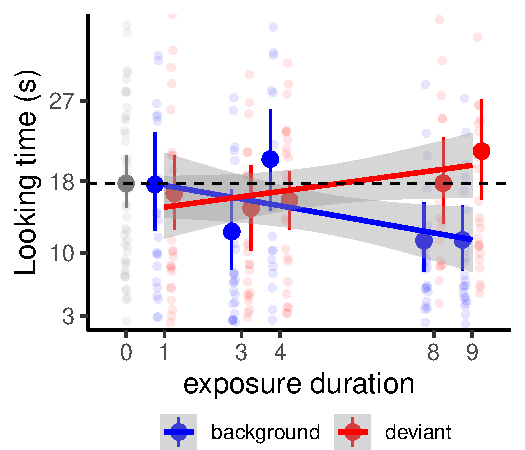
\includegraphics{figs/infant_results-1} \hfill{}

\caption[Looking times to background and deviant test trials as a function of exposure duration]{Looking times to background and deviant test trials as a function of exposure duration. We find evidence of habituation and novelty prefences, but not familiarity preferences. Y-axis is log-transformed to reflect transformation of looking times in mixed effects models. Grey data and dashed line show baseline looking times without familiarization.}\label{fig:infant_results}
\end{figure}
\end{CodeChunk}

\begin{table*}[t]
\centering
\begin{tabular}{lrrrrrr}
  \hline
 Predictor & Coefficient & Std error & t & df & p value \\ 
  \hline
(Intercept) & 2.79 & 0.11 & 25.13 & 179.98 & \textless{ 0.001} \\ 
  \textbf{Exposure duration} & -2.94 & 0.90 & -3.253 & 246.14 & 0.001 \\ 
  \textbf{Squared exposure duration} & 0.70 & 0.90 & 0.78 & 244.54 & 0.438 \\ 
  \textbf{Novelty} & 0.19 & 0.09 & 2.16 & 245.72 & 0.031 \\ 
  \textbf{Block number} & -0.11 & 0.02 & -4.54 & 248.53 & \textless{ 0.001} \\ 
  \textbf{Exposure duration} : \textbf{Novelty} & 4.93 & 1.59 & 3.10 & 250.18 & 0.002 \\ 
  \textbf{Squared exposure duration} : \textbf{Novelty} & 0.23 & 1.63 & 0.14 & 250.91 & 0.889 \\ 
   \hline
\end{tabular}
\caption{Mixed effects model results testing for a non-linearity in infant looking times.}\label{wrap-tab:1}
\end{table*}

\hypertarget{discussion}{%
\section{Discussion}\label{discussion}}

Overall, we developed a new looking time paradigm for infants and
preschoolers which tests the relationship between exposure duration and
the duration of attention, within-subjects. Using this paradigm, we
found evidence for habituation and novelty preferences across all ages
tested. In contrast, despite prematurely interrupting familiarization to
induce partial encoding, we failed to find attentional preferences for
familiar stimuli in either preschoolers or infants. Limited exposure did
not lead to familiarity preferences.

Both the presence of habituation and novelty preferences and the absence
of familiarity preferences were consistent across age groups (and
similar to previous results in adults), suggesting developmental
continuity of the dynamics of attention in this paradigm. For simple
visual events presented sequentially, the decision of how long to look
at a stimulus, and when to look away, can therefore be explained by a
simple information gain model, like the one presented in Cao et al.
(2022), across the lifespan.

Our failure to find familiarity preferences, in a within-subjects design
targeting partial encoding, should generate caution when inferring
familiarity preferences, post-hoc, in similar experiments. Note, though,
that the absence of familiarity preferences in our results does not rule
out their existence, in our paradigm or in general.

First, familiarity preferences may be more subtle than novelty
preferences, so that the statistical power that is needed to find
familiarity preferences is higher than that achieved in the current
study. A current large-scale study by the ManyBabies consortium which
aims to test the predictions made by H\&A may give insight into this
possibility (Kosie et al., 2023).

Second, evoking familiarity preferences may depend on the presentation
mode of stimuli: In our studies participants saw one stimulus, familiar
or novel, at a time. By contrast, many studies reporting familiarity
preferences follow a preferential looking set-up in which infants are
presented with both familiar and novel stimuli simultaneously, and their
relative looking time to each is recorded (Roder, Bushnell, \&
Sasseville, 2000; Rose et al., 1982; Thiessen \& Saffran, 2003).
Familiarity preferences could arise due to the \emph{recognition} of a
familiar stimulus among other stimuli, in which case the current
paradigm would not be suited to detect them (though see Gustafsson et
al., 2021).

Third, affective processes might drive familiarity preferences. The
``mere exposure effect'' is widely documented in social psychology:
brief exposure to a particular stimulus can be sufficient to induce
positive affect associated with that stimulus (Montoya, Horton, Vevea,
Citkowicz, \& Lauber, 2017; Zajonc, 1968). Therefore, it is possible
that familiarity preferences arise in infants when the familiar stimulus
evokes positive affect. Including measurements that more directly tap
into liking, such as reaching or pointing (Powell, 2022; Woo, Tan, \&
Hamlin, 2022), and relating them to looking time, may help isolate the
contribution of affect in familiarity preferences.

Finally, and most importantly, the learning problem that people are
solving likely plays a critical role in whether they will exhibit
familiarity preferences. This context-dependence is reflected in
meta-analyses investigating familiarity preferences in different
paradigms. For example, when tested on word segmentation in their native
language, infants show a persistent preference for familiar stimuli
throughout the first year (Bergmann \& Cristia, 2016). In contrast, when
tested on statistical learning of novel words, infants show a consistent
preference for novel stimuli, from 4-month- to 11 months of age (Black
\& Bergmann, 2017). These seemingly contradictory results highlight the
need for theories that formalize accounts of how the learning problem
influences optimal attention. Dubey \& Griffiths (2020) give an example
if such a formal account by showing that when past and present events
are correlated, a tendency to attend to familiar events may arise to
prepare for the most likely future events, while in uncorrelated
environments, novelty preferences are optimal (under some assumptions).
Similarly, in a rational analysis of attentional preferences, Cao et al.
(2022) show that ideal learners attempting to maximize their expected
information gain consistently seek novelty when trying to learn a single
concept. But it is possible that once the learning goal or constraints
on learning change e.g.~by attempting to learn hierarchical concepts or
imposing switch costs on learning new concepts, optimal
information-seeking may include a phase of attending to familiar
stimuli.

\hypertarget{conclusion}{%
\section{Conclusion}\label{conclusion}}

In conclusion, we find robust evidence for habituation and novelty
preferences in preschoolers and infants. In the same paradigms, we find
no evidence for familiarity preferences, despite attempting to impose
partial encoding through a new experimental paradigm in which we
manipulate exposure duration within-subjects. Our findings suggest that
familiarity preferences do not necessarily arise after limited exposure
to stimuli, so post-hoc inferences of familiarity preferences in infant
looking time data should be made with care. Instead, we conclude that
developmental psychology needs formal models to make specific
predictions for the conditions under which infants will, and will not,
show familiarity preferences, that can then be rigorously tested in
experiments.

\hypertarget{references}{%
\section{References}\label{references}}

\setlength{\parindent}{-0.1in} 
\setlength{\leftskip}{0.125in}

\noindent

\hypertarget{refs}{}
\begin{CSLReferences}{1}{0}
\leavevmode\vadjust pre{\hypertarget{ref-aslin2007s}{}}%
Aslin, R. N. (2007). What's in a look? \emph{Developmental Science},
\emph{10}(1), 48--53.

\leavevmode\vadjust pre{\hypertarget{ref-baillargeon1985object}{}}%
Baillargeon, R., Spelke, E. S., \& Wasserman, S. (1985). Object
permanence in five-month-old infants. \emph{Cognition}, \emph{20}(3),
191--208.

\leavevmode\vadjust pre{\hypertarget{ref-bergmann2016development}{}}%
Bergmann, C., \& Cristia, A. (2016). Development of infants'
segmentation of words from native speech: A meta-analytic approach.
\emph{Developmental Science}, \emph{19}(6), 901--917.

\leavevmode\vadjust pre{\hypertarget{ref-black2017quantifying}{}}%
Black, A., \& Bergmann, C. (2017). Quantifying infants' statistical word
segmentation: A meta-analysis. In \emph{39th annual meeting of the
cognitive science society} (pp. 124--129). Cognitive Science Society.

\leavevmode\vadjust pre{\hypertarget{ref-cao2022habituation}{}}%
Cao, A., Raz, G., Saxe, R., \& Frank, M. C. (2022). Habituation reflects
optimal exploration over noisy perceptual samples. \emph{Topics in
Cognitive Science}.

\leavevmode\vadjust pre{\hypertarget{ref-cyr2013development}{}}%
Cyr, M., \& Shi, R. (2013). Development of abstract grammatical
categorization in infants. \emph{Child Development}, \emph{84}(2),
617--629.

\leavevmode\vadjust pre{\hypertarget{ref-dubey2020reconciling}{}}%
Dubey, R., \& Griffiths, T. L. (2020). Reconciling novelty and
complexity through a rational analysis of curiosity. \emph{Psychological
Review}, \emph{127}(3), 455.

\leavevmode\vadjust pre{\hypertarget{ref-dweck2017needs}{}}%
Dweck, C. S. (2017). From needs to goals and representations:
Foundations for a unified theory of motivation, personality, and
development. \emph{Psychological Review}, \emph{124}(6), 689.

\leavevmode\vadjust pre{\hypertarget{ref-erel2022icatcher}{}}%
Erel, Y., Shannon, K. A., Scott, K., Cao, P., Tan, X., Hart, P. K.,
\ldots{} Liu, S. (in press). iCatcher+: Robust and automated annotation
of infant gaze from videos collected in the lab and online.
\emph{Advances in Methods and Practices in Psychological Sciences}.

\leavevmode\vadjust pre{\hypertarget{ref-fantz1963pattern}{}}%
Fantz, R. L. (1963). Pattern vision in newborn infants. \emph{Science},
\emph{140}(3564), 296--297.

\leavevmode\vadjust pre{\hypertarget{ref-guest2021computational}{}}%
Guest, O., \& Martin, A. E. (2021). How computational modeling can force
theory building in psychological science. \emph{Perspectives on
Psychological Science}, \emph{16}(4), 789--802.

\leavevmode\vadjust pre{\hypertarget{ref-gustafsson2021visual}{}}%
Gustafsson, E., Francoeur, C., Blanchette, I., \& Sirois, S. (2021).
Visual exploration in adults: Habituation, mere exposure, or optimal
level of arousal? \emph{Learning \& Behavior}, 1--9.

\leavevmode\vadjust pre{\hypertarget{ref-haith1980rules}{}}%
Haith, M. M. (1980). \emph{Rules that babies look by: The organization
of newborn visual activity}. Lawrence Erlbaum Associates.

\leavevmode\vadjust pre{\hypertarget{ref-hunter1988multifactor}{}}%
Hunter, M. A., \& Ames, E. W. (1988). A multifactor model of infant
preferences for novel and familiar stimuli. \emph{Advances in Infancy
Research}.

\leavevmode\vadjust pre{\hypertarget{ref-hunter1983effects}{}}%
Hunter, M. A., Ames, E. W., \& Koopman, R. (1983). Effects of stimulus
complexity and familiarization time on infant preferences for novel and
familiar stimuli. \emph{Developmental Psychology}, \emph{19}(3), 338.

\leavevmode\vadjust pre{\hypertarget{ref-johnson2009abstract}{}}%
Johnson, S. P., Fernandes, K. J., Frank, M. C., Kirkham, N., Marcus, G.,
Rabagliati, H., \& Slemmer, J. A. (2009). Abstract rule learning for
visual sequences in 8-and 11-month-olds. \emph{Infancy}, \emph{14}(1),
2--18.

\leavevmode\vadjust pre{\hypertarget{ref-karni2022}{}}%
Karni, G., Mattar, M. G., Emberson, L., \& Daw, N. (2022). \emph{A
rational information gathering account of infant exploratory behavior.
{[}Poster presentation{]}. RLDM}.

\leavevmode\vadjust pre{\hypertarget{ref-kidd2012goldilocks}{}}%
Kidd, C., Piantadosi, S. T., \& Aslin, R. N. (2012). The goldilocks
effect: Human infants allocate attention to visual sequences that are
neither too simple nor too complex. \emph{PloS One}, \emph{7}(5),
e36399.

\leavevmode\vadjust pre{\hypertarget{ref-kosie2023manybabies}{}}%
Kosie, J., Zettersten, M., Abu-Zhaya, R., Amso, D., Babineau, M.,
Baumgartne, H., et al.others. (2023). ManyBabies 5: A large-scale
investigation of the proposed shift from familiarity preference to
novelty preference in infant looking time.

\leavevmode\vadjust pre{\hypertarget{ref-montoya2017re}{}}%
Montoya, R. M., Horton, R. S., Vevea, J. L., Citkowicz, M., \& Lauber,
E. A. (2017). A re-examination of the mere exposure effect: The
influence of repeated exposure on recognition, familiarity, and liking.
\emph{Psychological Bulletin}, \emph{143}(5), 459.

\leavevmode\vadjust pre{\hypertarget{ref-powell2022adopted}{}}%
Powell, L. J. (2022). Adopted utility calculus: Origins of a concept of
social affiliation. \emph{Perspectives on Psychological Science},
\emph{17}(5), 1215--1233.

\leavevmode\vadjust pre{\hypertarget{ref-raz2020learning}{}}%
Raz, G., \& Saxe, R. (2020). Learning in infancy is active, endogenously
motivated, and depends on the prefrontal cortices. \emph{Annual Review
of Developmental Psychology}, \emph{2}, 247--268.

\leavevmode\vadjust pre{\hypertarget{ref-roder2000infants}{}}%
Roder, B. J., Bushnell, E. W., \& Sasseville, A. M. (2000). Infants'
preferences for familiarity and novelty during the course of visual
processing. \emph{Infancy}, \emph{1}(4), 491--507.

\leavevmode\vadjust pre{\hypertarget{ref-rose1982familiarity}{}}%
Rose, S. A., Gottfried, A. W., Melloy-Carminar, P., \& Bridger, W. H.
(1982). Familiarity and novelty preferences in infant recognition
memory: Implications for information processing. \emph{Developmental
Psychology}, \emph{18}(5), 704.

\leavevmode\vadjust pre{\hypertarget{ref-scott2017lookit}{}}%
Scott, K., \& Schulz, L. (2017). Lookit (part 1): A new online platform
for developmental research. \emph{Open Mind}, \emph{1}(1), 4--14.

\leavevmode\vadjust pre{\hypertarget{ref-sirois2002models}{}}%
Sirois, S., \& Mareschal, D. (2002). Models of habituation in infancy.
\emph{Trends in Cognitive Sciences}, \emph{6}(7), 293--298.

\leavevmode\vadjust pre{\hypertarget{ref-smaldino2020translate}{}}%
Smaldino, P. E. (2020). How to translate a verbal theory into a formal
model. \emph{Social Psychology}.

\leavevmode\vadjust pre{\hypertarget{ref-thiessen2003cues}{}}%
Thiessen, E. D., \& Saffran, J. R. (2003). When cues collide: Use of
stress and statistical cues to word boundaries by 7-to 9-month-old
infants. \emph{Developmental Psychology}, \emph{39}(4), 706.

\leavevmode\vadjust pre{\hypertarget{ref-woo2022human}{}}%
Woo, B. M., Tan, E., \& Hamlin, J. K. (2022). Human morality is based on
an early-emerging moral core. \emph{Annual Review of Developmental
Psychology}, \emph{4}, 41--61.

\leavevmode\vadjust pre{\hypertarget{ref-zajonc1968attitudinal}{}}%
Zajonc, R. B. (1968). Attitudinal effects of mere exposure.
\emph{Journal of Personality and Social Psychology}, \emph{9}(2p2), 1.

\end{CSLReferences}

\bibliographystyle{apacite}


\end{document}
